%----------------------------------------------------------------------------------------
% Einführung in das Wissenschaftliche Arbeiten 
% Report LaTeX template (English)
% Interactive Graphics and Simulation Group
% University of Innsbruck
%----------------------------------------------------------------------------------------

\documentclass[11pt,a4paper]{article}

%----------------------------------------------------------------------------------------
% Include required packages
\usepackage{graphicx}
\usepackage{amsmath}

\usepackage[english]{babel}
%\usepackage[ngerman]{babel}

\usepackage[utf8x]{inputenc}
\usepackage[T1]{fontenc}
\usepackage{float}

\usepackage[left=2.7cm, right=2.7cm, top=3cm]{geometry}

\usepackage{url}

%----------------------------------------------------------------------------------------
% Start document

\begin{document}


%----------------------------------------------------------------------------------------
% Title page
%----------------------------------------------------------------------------------------

\begin{titlepage} % User-defined title page

\begin{center}

\includegraphics[width=1.2cm]{images/uibk}

\begin{large}
Leopold-Franzens-Universität Innsbruck\\[5mm]
Institute of Computer Science\\
Interactive Graphics and Simulation Group\\[25mm]
\end{large}

{\LARGE \bf Raytracing Project}

Advanced Computer Graphics\\ 
Documentation\\[15mm]

Phillip Mildenberger\\
Stefan Spiss\\
Cem Okulmus\\[35mm]

advised by\\
Savoye Yann Pierre, PhD\\[10mm]

\vfill

Innsbruck, \today
\end{center}

\end{titlepage}


%----------------------------------------------------------------------------------------
% Main body
%----------------------------------------------------------------------------------------

\section{Introduction}
For this project we had to implement certain advanced features based on smallPT. Every student in one group had to implement at least one main feature. In our group we chose Motion Blur (by Cem Okulmus), Depth of Field (by Stefan Spiss) and Specular/Texture/Normal Mapping (by Philipp Mildenberger). Additionally in our project extra features were implemented, such as: Acceleration Structures (by Philipp Mildenberger), simple Camera Control (by Stefan Spiss).

\section{Technical Overview}
SmallPT was extended by .obj import and complex geometry now supporting triangle meshes. Additionally a bounding volume hierarchy (BVH) is used to speed up the calculation of complex scenes. Texture-/normal- and specular-mapping is implemented to generate more realistic images. Furthermore to simulate a camera, Depth of Field provides correct blurring of objects that are not in focus. It's now also easy possible to move the camera around, change it's focal distance, it's field of view and it's aperture size. To capture movements in still pictures the effect of Motion Blur is approached by simulating the aperture shutter speed.

\section{Implementation Detail}
In this section we will give a short explanation how every feature was implemented. All of these are extensions of the smallPT code. 

\subsection{Motion Blur}
If we want to simulate motion using multiple ray-traced images, we will observe a strobing effect, since a camera always blurs a moving object. This is called Motion Blur.
As was explained during the lecture, the basic idea behind this effect is that we want to distribute the rays not in space but in time. For this we usually also want to have some sort of animation, otherwise the effect wouldn't show. This method was first detailed by Cook et al. \cite{Cook:1984}.
Since smallPT also uses a distribution over space, only an extension of this was needed.
The rays are uniformally distributed over time, with equal weight for all time steps. So the four subpixel samples are assigned different time scenes and the average is returned.
This simulates an object that's moving with no acceleration. 

\subsection{Depth of Field}
In standard smallPT the pinhole camera model is used. So everything in the scene is in focus. Normal cameras always have a Depth of Field, which means that only objects in a specific distance are in focus. Everything else is blurred depending on the distance to the focal point. In the project implementation the Thin-Lens model is used. For this the ray direction is changed. Rays are shot not only from one camera position, but distributed over the aperture circle. As target for the rays the focal plane is used instead of the image plane. The focal plane is perpendicular to the camera and at the position of the focal point. See Figure~\ref{fig:1}
\\
\\
Furthermore for general information about Depth of Field following sources were used:
\begin{itemize}
\item
A realistic camera model for computer graphics, \cite{kolb1995realistic}
\item
Camera models and optical systems used in computer graphics: part I, object-based techniques, \cite{barsky2003camera}
\item
Algorithms for rendering depth of field effects in computer graphics, \cite{barsky2008algorithms}

\end{itemize}

\begin{figure}[h]
\begin{center}
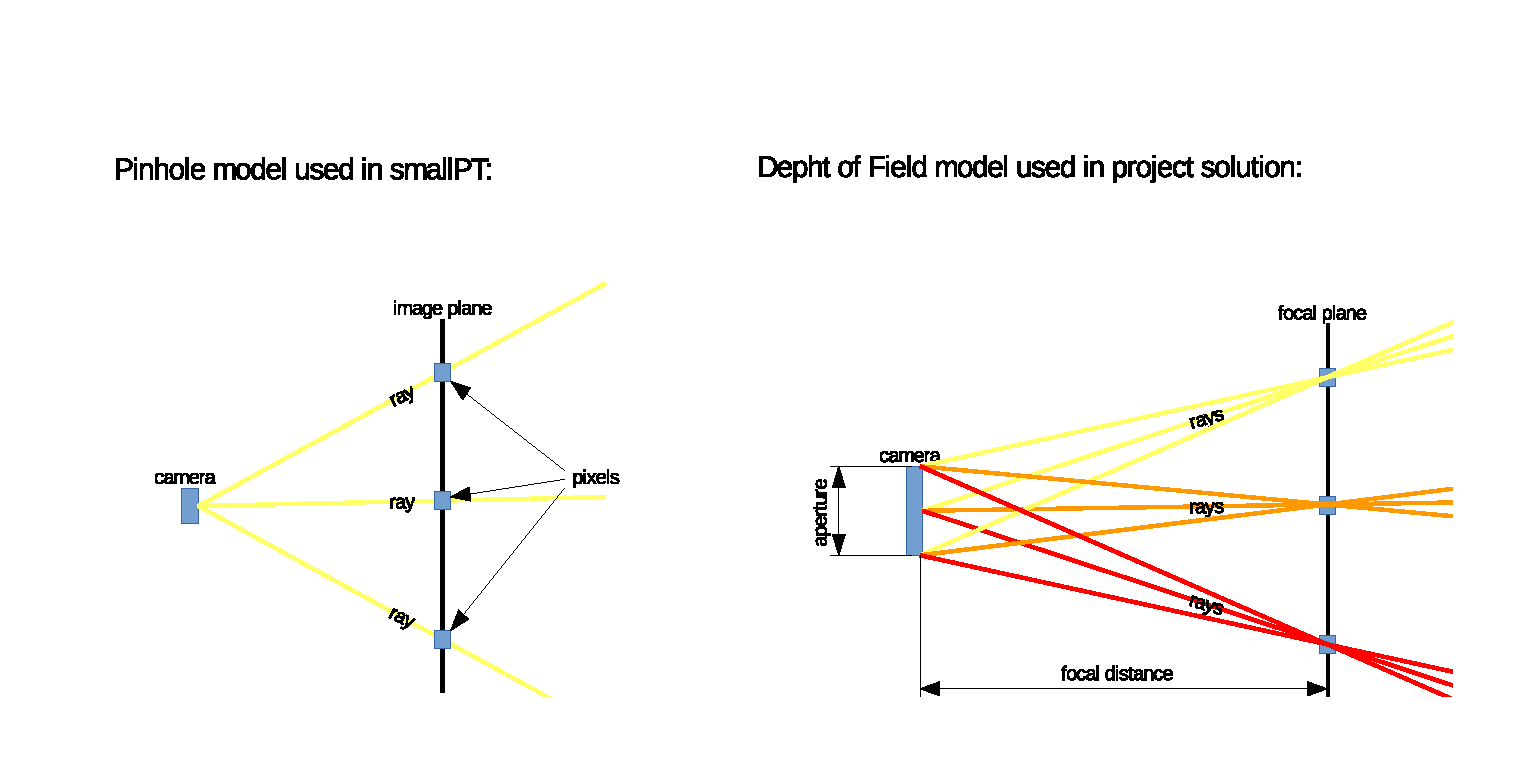
\includegraphics[trim=40 30 60 60, clip=true, scale=0.6]{images/pinholeVsDepthOfField}
\caption[Pinhole implementation vs Thin Lens implementation]{This figure shows the simplified camera models. On the left the model used in smallPT, on the right the model for the project solution can be seen. (\textbf{Recreation from:} online tutorial from Steve Harvey, \cite{link:Harvey})}
\label{fig:1}
\end{center}
\end{figure}

\subsection{Specular/Texture/Normal Mapping}
UV mapping from obj-files is supported, including import of color, specular and normal data.
For specular mapping a new material had to be created: Glossy surface. It's used to supply specular data with a texture. The normal mapping is changing the intersection normal for depending on the texture for the surface. 
For every intersection we return a special intersection structure, additionally containing the needed data for specular/normal/texture mapping. 

\subsection{Acceleration Structures}
To accelerate the intersection of complex triangle-meshes in smallPT, we implemented different acceleration structures. 
The first is just simple approach: A bounding box is put around every object, and the intersection function first checks every bounding box and only continues if one was hit.
The second is a  Bounding Volume Hierarchy (BVH). An octree is used to build up the hierarchy recursively: Every object is inserted using its centroid. From these objects, using bottom-up traversal, the BVH is constructed.
\\
\\
For the implementation of Acceleration Structures mainly the website scratchapixel \cite{link:scratch}
was used.

\subsection{Camera Control}
In smallPT the camera settings are hard-coded (fixed position, direction, field of view). The project solution uses a additional camera class which implements all camera aspects like position, direction, field of view and focal distance. Now it is very simple to render a scene from different perspectives with different camera settings.

\section{Results}
The following images are rendered with our program showing different features of it.


\begin{itemize}
\item
Motion Blur:\\
\begin{figure}[H]
\begin{center}
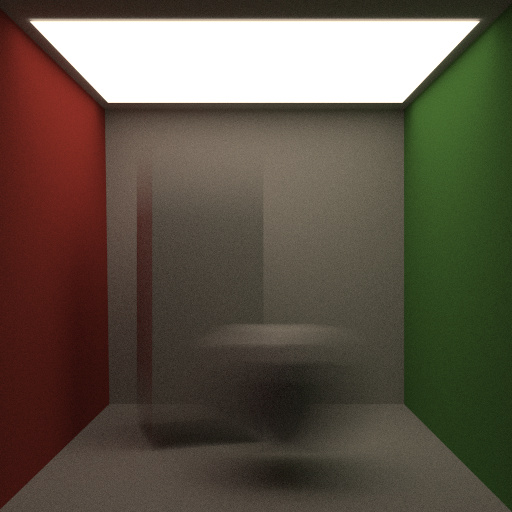
\includegraphics[scale=0.4]{images/motionBlur560spp}
\caption[Picture showing Motion Blur]{Picture rendered just with Motion Blur}
\label{fig:2}
\end{center}
\end{figure}

\item
Depth of Field and changed camera settings:\\
\begin{figure}[H]
\begin{center}
\begin{minipage}[b]{7.5 cm}
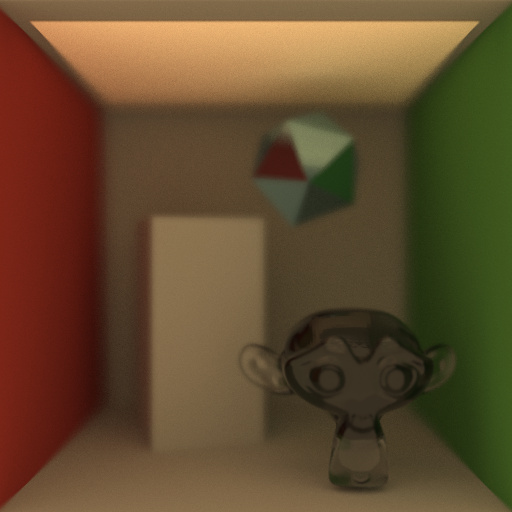
\includegraphics[scale=0.4]{images/DepthOfFieldFront1096spp}
\label{fig:3}
\end{minipage}
\begin{minipage}[b]{7.5 cm}
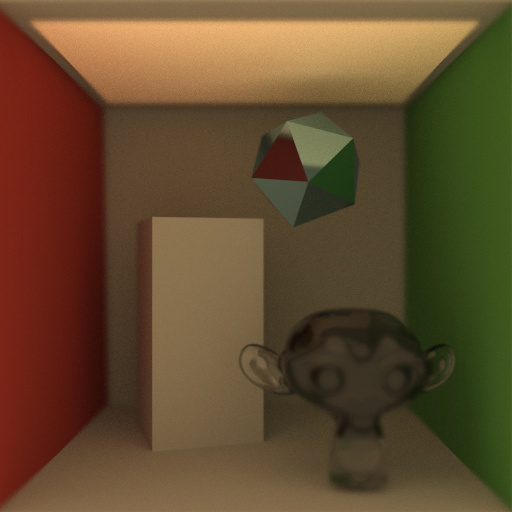
\includegraphics[scale=0.4]{images/DepthOfFieldBack1000spp}
\label{fig:4}
\end{minipage}
\caption[Picture showing Depth of Field]{Picture rendered just with Depth of Field}
\end{center}
\end{figure}

\item
Specular/Texture/Normal Mapping:\\
\begin{figure}[H]
\begin{center}
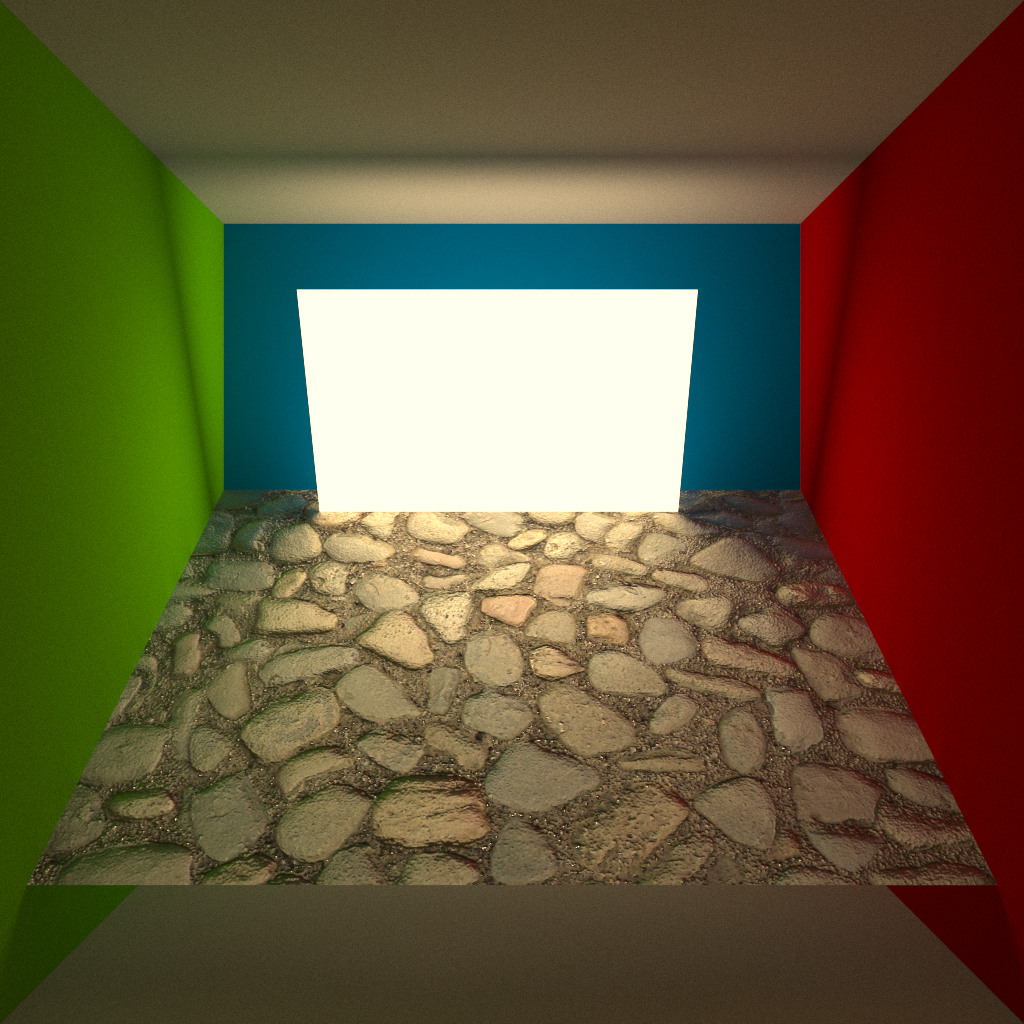
\includegraphics[scale=0.2]{images/bumbmapped1000spp}
\caption[Picture showing Specular/Texture/Normal Mapping]{Picture rendered with Specular/Texture/Normal Mapping}
\label{fig:5}
\end{center}
\end{figure}

\begin{figure}[H]
\begin{center}
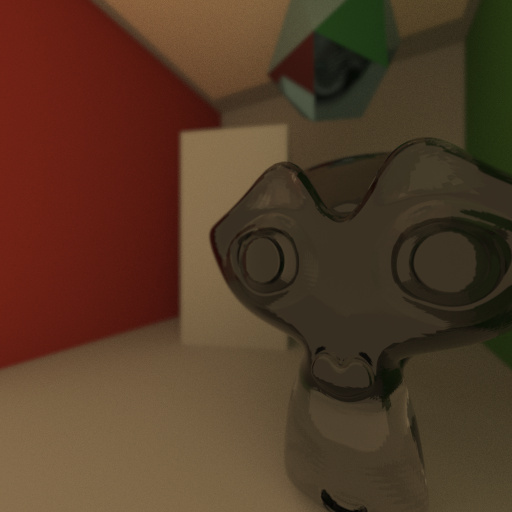
\includegraphics[scale=0.4]{images/changedCameraPosition1000spp}
\caption[Picture showing changed camera settings]{Picture rendered with changed camera settings}
\label{fig:6}
\end{center}
\end{figure}

\item
Putting all together:\\
\begin{figure}[H]
\begin{center}
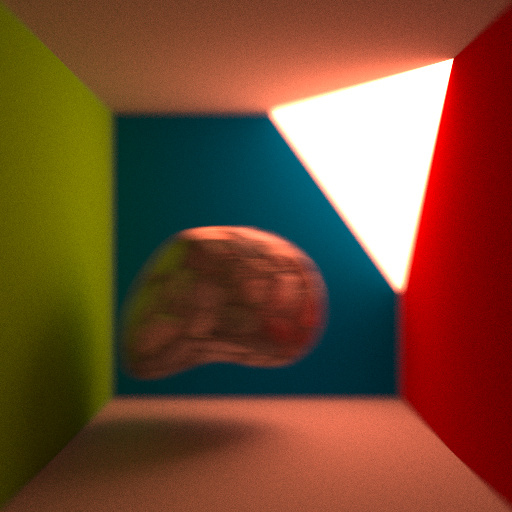
\includegraphics[scale=0.4]{images/deformedstone2100spp}
\caption[Picture showing all effects]{Picture showing all effects}
\label{fig:7}
\end{center}
\end{figure}

\end{itemize}

%----------------------------------------------------------------------------------------
% Bibliography
%----------------------------------------------------------------------------------------

\bibliographystyle{plain}
\bibliography{EWA_literature}

\end{document}
